\documentclass{ximera}

\title{Graphics}

\begin{document}
\begin{abstract}
  Embed pictures in Ximera activities.
\end{abstract}
\maketitle

We've seen basic ways to include JPGs, PNGs, and PDFs using
\verb!\includegraphics!. However, this is not the preferred way to include
graphics. Moreover, there are considerations for positioning of the graphics.

\section{Positioning graphics}

In \LaTeX\ it is common to write images in the \verb!figure! environment. We
choose not to use this because \verb!figure! `floats' the images for `optimal'
page layout. We are not concerned with page layout. When working online, the
page is essentially infinite in length. Moreover, the \textit{consumers} of the
content we create are \textit{students}. Students are also unconcerned with
awkward page layout. Students prefer to see the image exactly when it is
mentioned. With this said, we suggest wrapping all images in either a
\verb!center! environment or an (Ximera-specific) \verb!image! environment.
The environment \verb!image! centers and automatically scales the contents.  If
an author finds themselves printing to various page-sizes, \verb!image! might
be preferred. Moreover, \verb!image! can be redefined globally to act
identically to \verb!center!, but \verb!center! cannot be redefined.

If you use \verb!center!, you would write something like:
\begin{verbatim}
\begin{center}

\includegraphics[width=5cm]{missionPatch.jpg}
\end{center}
\end{verbatim}
If you use \verb!image!, you would write something like:
\begin{verbatim}
\begin{image}

\includegraphics[width=5cm]{missionPatch.jpg}
\end{image}
\end{verbatim}

The disadvantage of using \verb!\includegraphics! is that you need to handle
the paths to the images in some way. However, we now suggest you use a global
graphics path: You may store all your graphics inside \verb!\xmPictures!. 
This means that any required \verb!*.jpg!, \verb!*.png!, and \verb!*.pdf! can
be found, assuming your file isn't nested too deep.
Moreover, we've set up the \verb!.gitignore! to \text{not ignore} \verb!*.jpg!,
\verb!*.png!, and \verb!*.pdf! when they are placed in the \verb!xmPictures!
directory. Finally, while this is currently the \textit{easiest} method for
adding graphics in Ximera, it might be better if all graphics were placed at
the level of the source file, and then a soft link (using the terminal) could
be made to the
\verb!xmPictures! directory. The advantage here being that if someone wants to
borrow your material, everything they need is in the same folder.

With this said, TikZ is the preferred method for graphics because code, found
in the Ximera \LaTeX\ file, generates the image. No need to worry about
graphics paths.

\section{TikZ is the preferred method for graphics}

Most of TikZ is supported,
and these are rendered as PNGs online.
For example the image below:
\begin{image}
  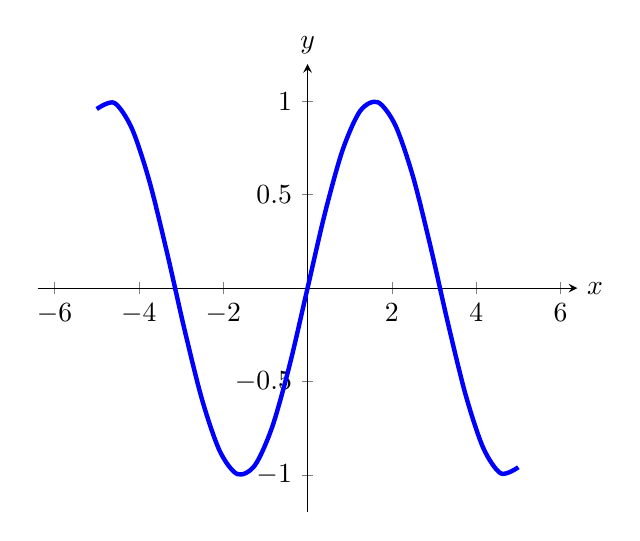
\begin{tikzpicture}
    \begin{axis}[
        xmin=-6.4,
        xmax=6.4,
        ymin=-1.2,
        ymax=1.2,
        axis lines=center,
        xlabel=$x$,
        ylabel=$y$,
        every axis y label/.style={at=(current axis.above
            origin),anchor=south},
        every axis x label/.style={at=(current axis.right of
            origin),anchor=west},
      ]
      \addplot [ultra thick, blue, smooth] {sin(deg(x))};
    \end{axis}
  \end{tikzpicture}
\end{image}
was generated via
\begin{verbatim}
\begin{image}
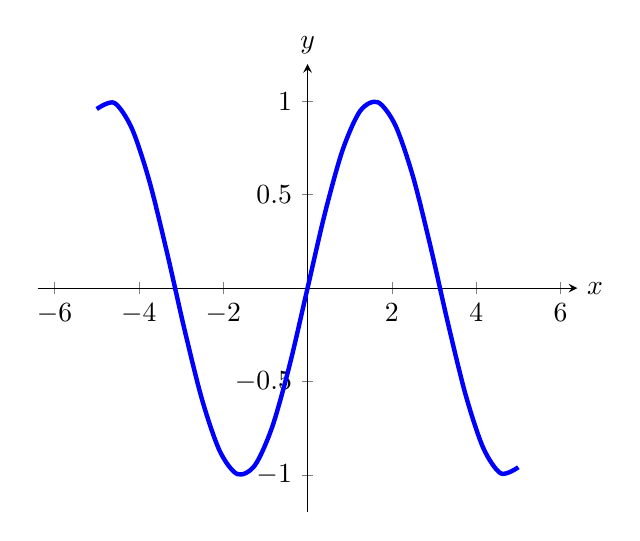
\begin{tikzpicture}
  \begin{axis}[
  xmin=-6.4,
  xmax=6.4,
  ymin=-1.2,
  ymax=1.2,
  axis lines=center,
  xlabel=$x$,
  ylabel=$y$,
  every axis y label/.style=
    {at=(current axis.above origin),anchor=south},
  every axis x label/.style=
    {at=(current axis.right of origin),anchor=west},
  ]
\addplot [ultra thick, blue, smooth] {sin(deg(x))};
\end{axis}
\end{tikzpicture}
\end{image}
\end{verbatim}
When you use TikZ for graphics, you don't need to worry about \verb!\graphicspath!.



\end{document}